\documentclass[]{book}
\usepackage{lmodern}
\usepackage{amssymb,amsmath}
\usepackage{ifxetex,ifluatex}
\usepackage{fixltx2e} % provides \textsubscript
\ifnum 0\ifxetex 1\fi\ifluatex 1\fi=0 % if pdftex
  \usepackage[T1]{fontenc}
  \usepackage[utf8]{inputenc}
\else % if luatex or xelatex
  \ifxetex
    \usepackage{mathspec}
  \else
    \usepackage{fontspec}
  \fi
  \defaultfontfeatures{Ligatures=TeX,Scale=MatchLowercase}
\fi
% use upquote if available, for straight quotes in verbatim environments
\IfFileExists{upquote.sty}{\usepackage{upquote}}{}
% use microtype if available
\IfFileExists{microtype.sty}{%
\usepackage{microtype}
\UseMicrotypeSet[protrusion]{basicmath} % disable protrusion for tt fonts
}{}
\usepackage[margin=1in]{geometry}
\usepackage{hyperref}
\hypersetup{unicode=true,
            pdftitle={WHY WE HAVE TO CODE},
            pdfauthor={Ujang Fahmi and Canggih Puspo Wibowo},
            pdfborder={0 0 0},
            breaklinks=true}
\urlstyle{same}  % don't use monospace font for urls
\usepackage{natbib}
\bibliographystyle{apalike}
\usepackage{color}
\usepackage{fancyvrb}
\newcommand{\VerbBar}{|}
\newcommand{\VERB}{\Verb[commandchars=\\\{\}]}
\DefineVerbatimEnvironment{Highlighting}{Verbatim}{commandchars=\\\{\}}
% Add ',fontsize=\small' for more characters per line
\usepackage{framed}
\definecolor{shadecolor}{RGB}{248,248,248}
\newenvironment{Shaded}{\begin{snugshade}}{\end{snugshade}}
\newcommand{\AlertTok}[1]{\textcolor[rgb]{0.94,0.16,0.16}{#1}}
\newcommand{\AnnotationTok}[1]{\textcolor[rgb]{0.56,0.35,0.01}{\textbf{\textit{#1}}}}
\newcommand{\AttributeTok}[1]{\textcolor[rgb]{0.77,0.63,0.00}{#1}}
\newcommand{\BaseNTok}[1]{\textcolor[rgb]{0.00,0.00,0.81}{#1}}
\newcommand{\BuiltInTok}[1]{#1}
\newcommand{\CharTok}[1]{\textcolor[rgb]{0.31,0.60,0.02}{#1}}
\newcommand{\CommentTok}[1]{\textcolor[rgb]{0.56,0.35,0.01}{\textit{#1}}}
\newcommand{\CommentVarTok}[1]{\textcolor[rgb]{0.56,0.35,0.01}{\textbf{\textit{#1}}}}
\newcommand{\ConstantTok}[1]{\textcolor[rgb]{0.00,0.00,0.00}{#1}}
\newcommand{\ControlFlowTok}[1]{\textcolor[rgb]{0.13,0.29,0.53}{\textbf{#1}}}
\newcommand{\DataTypeTok}[1]{\textcolor[rgb]{0.13,0.29,0.53}{#1}}
\newcommand{\DecValTok}[1]{\textcolor[rgb]{0.00,0.00,0.81}{#1}}
\newcommand{\DocumentationTok}[1]{\textcolor[rgb]{0.56,0.35,0.01}{\textbf{\textit{#1}}}}
\newcommand{\ErrorTok}[1]{\textcolor[rgb]{0.64,0.00,0.00}{\textbf{#1}}}
\newcommand{\ExtensionTok}[1]{#1}
\newcommand{\FloatTok}[1]{\textcolor[rgb]{0.00,0.00,0.81}{#1}}
\newcommand{\FunctionTok}[1]{\textcolor[rgb]{0.00,0.00,0.00}{#1}}
\newcommand{\ImportTok}[1]{#1}
\newcommand{\InformationTok}[1]{\textcolor[rgb]{0.56,0.35,0.01}{\textbf{\textit{#1}}}}
\newcommand{\KeywordTok}[1]{\textcolor[rgb]{0.13,0.29,0.53}{\textbf{#1}}}
\newcommand{\NormalTok}[1]{#1}
\newcommand{\OperatorTok}[1]{\textcolor[rgb]{0.81,0.36,0.00}{\textbf{#1}}}
\newcommand{\OtherTok}[1]{\textcolor[rgb]{0.56,0.35,0.01}{#1}}
\newcommand{\PreprocessorTok}[1]{\textcolor[rgb]{0.56,0.35,0.01}{\textit{#1}}}
\newcommand{\RegionMarkerTok}[1]{#1}
\newcommand{\SpecialCharTok}[1]{\textcolor[rgb]{0.00,0.00,0.00}{#1}}
\newcommand{\SpecialStringTok}[1]{\textcolor[rgb]{0.31,0.60,0.02}{#1}}
\newcommand{\StringTok}[1]{\textcolor[rgb]{0.31,0.60,0.02}{#1}}
\newcommand{\VariableTok}[1]{\textcolor[rgb]{0.00,0.00,0.00}{#1}}
\newcommand{\VerbatimStringTok}[1]{\textcolor[rgb]{0.31,0.60,0.02}{#1}}
\newcommand{\WarningTok}[1]{\textcolor[rgb]{0.56,0.35,0.01}{\textbf{\textit{#1}}}}
\usepackage{longtable,booktabs}
\usepackage{graphicx,grffile}
\makeatletter
\def\maxwidth{\ifdim\Gin@nat@width>\linewidth\linewidth\else\Gin@nat@width\fi}
\def\maxheight{\ifdim\Gin@nat@height>\textheight\textheight\else\Gin@nat@height\fi}
\makeatother
% Scale images if necessary, so that they will not overflow the page
% margins by default, and it is still possible to overwrite the defaults
% using explicit options in \includegraphics[width, height, ...]{}
\setkeys{Gin}{width=\maxwidth,height=\maxheight,keepaspectratio}
\IfFileExists{parskip.sty}{%
\usepackage{parskip}
}{% else
\setlength{\parindent}{0pt}
\setlength{\parskip}{6pt plus 2pt minus 1pt}
}
\setlength{\emergencystretch}{3em}  % prevent overfull lines
\providecommand{\tightlist}{%
  \setlength{\itemsep}{0pt}\setlength{\parskip}{0pt}}
\setcounter{secnumdepth}{5}
% Redefines (sub)paragraphs to behave more like sections
\ifx\paragraph\undefined\else
\let\oldparagraph\paragraph
\renewcommand{\paragraph}[1]{\oldparagraph{#1}\mbox{}}
\fi
\ifx\subparagraph\undefined\else
\let\oldsubparagraph\subparagraph
\renewcommand{\subparagraph}[1]{\oldsubparagraph{#1}\mbox{}}
\fi

%%% Use protect on footnotes to avoid problems with footnotes in titles
\let\rmarkdownfootnote\footnote%
\def\footnote{\protect\rmarkdownfootnote}

%%% Change title format to be more compact
\usepackage{titling}

% Create subtitle command for use in maketitle
\newcommand{\subtitle}[1]{
  \posttitle{
    \begin{center}\large#1\end{center}
    }
}

\setlength{\droptitle}{-2em}

  \title{WHY WE HAVE TO CODE}
    \pretitle{\vspace{\droptitle}\centering\huge}
  \posttitle{\par}
  \subtitle{a CDC FISIPOL, UGM Workshop}
  \author{Ujang Fahmi and Canggih Puspo Wibowo}
    \preauthor{\centering\large\emph}
  \postauthor{\par}
      \predate{\centering\large\emph}
  \postdate{\par}
    \date{2018-10-18}

\usepackage{booktabs}
\usepackage{amsthm}
\makeatletter
\def\thm@space@setup{%
  \thm@preskip=8pt plus 2pt minus 4pt
  \thm@postskip=\thm@preskip
}
\makeatother

\usepackage{amsthm}
\newtheorem{theorem}{Theorem}[chapter]
\newtheorem{lemma}{Lemma}[chapter]
\theoremstyle{definition}
\newtheorem{definition}{Definition}[chapter]
\newtheorem{corollary}{Corollary}[chapter]
\newtheorem{proposition}{Proposition}[chapter]
\theoremstyle{definition}
\newtheorem{example}{Example}[chapter]
\theoremstyle{definition}
\newtheorem{exercise}{Exercise}[chapter]
\theoremstyle{remark}
\newtheorem*{remark}{Remark}
\newtheorem*{solution}{Solution}
\begin{document}
\maketitle

{
\setcounter{tocdepth}{1}
\tableofcontents
}
\hypertarget{pengantar}{%
\chapter*{Pengantar}\label{pengantar}}
\addcontentsline{toc}{chapter}{Pengantar}

Saat ini sumber data yang dapat digunakan baik untuk tujuan penelitian
maupun bisnis banyak tersedia di internet. Sayangnya, tidak semua orang
bisa memanfaatkannya. Terdapat beberapa kendala mengapa tidak semua
orang bisa mengekstrak pengetahuan dari sumber data yang cenderung lebih
murah dan sebenarnya mudah untuk di dapatkan tersebut. Salah satu sebab
utamanya kurangnya keterampilan untuk membuat alat untuk mengambilnya.
Dalam konteks ini adalah keterampilan untuk memanfaatkan open source,
salah satunya adalah R.

R merupakan salah satu open source yang saat ini cukup populer dan
banyak digunakan oleh berbagai organisasi dengan skala besar hingga
kecil. Pengguna R tersebar mulai dari perusahaan seperti Google dan
Facebook, pemerintahan, hingga usaha kecil menengah. Berdasarkan
definisi di laman resminya, R merupakan bahasa pemrograman untuk
mengolah data secara statistik. Dalam praktinya R juga banyak digunakan
untuk mengolah data tidak terstruktur, termasuk data dari media sosial.

Sayangnya, \emph{coding} diidentikan hanya dilakukan oleh anak teknik.
Hanya sedikit akademisi sosial yang memiliki kemampuan tersebut.
Padahal, akademisi sosial memiliki salah satu modal utama untuk bisa
membuat data menjadi lebih berarti, yaitu \emph{domain knowledge}.
Sebaliknya, hanya sedikit yang bisa \emph{coding} memiliki \emph{domain
knowledge} untuk bisa memanfaatkan informasi yang diekstrak dari data
dalam jumlah banyak. Dalam konteks ini, kolaborasi lintas disiplin ilmu
dapat menjadi salah satu solusi. Tapi, masing-masing pihak minimal
memiliki pengetahuan dan pemahaman dasar tentang cara kerja
masing-masing. Selain itu, akademisi sosial juga bisa belajar sendiri
dengan memanfaatkan berbagai sumber baik yang gratis maupun berbayar
yang saat ini banyak tersedia di Interent.

Melalui workshop ini, kami bertujuan untuk mengenalkan beberapa dasar
pengelolaan big data dengan menggunakan bahasa pemrograman R. Setelah
mengikuti workhshop, peserta diharapkan memiliki:

\begin{enumerate}
\def\labelenumi{\arabic{enumi}.}
\tightlist
\item
  Pengetahuan tentang bahasa pemrograman;
\item
  Pemahaman alur pengolahan big data; dan
\item
  Kemampuan untuk membuat skrip/menjalankan skrip untuk mendapatkan data
  dari internet
\end{enumerate}

Workshop ini terdiri dari beberapa kegiatan. \emph{Pertama}, penjelasan
tentang R dan Rstudio. \emph{Kedua}, memahami proses ekstraksi informasi
dari big data. \emph{Ketiga}, praktik mendapatkan dan mengeksplorasi
data dari twitter.

\hypertarget{r-dan-rstudio}{%
\chapter{\texorpdfstring{\texttt{R} dan
\texttt{Rstudio}}{R dan Rstudio}}\label{r-dan-rstudio}}

Sebelum melangkah lebih jauh, mungkin kita terlebih dahulu perlu
mengetahui apa itu bahasa pemrograman? apakah ia merupakan bahasa yang
berfungsi sama dengan bahasa yang kita gunakan sehari-hari? Menurut
\href{https://en.wikipedia.org/wiki/Programming_language}{Wikipedia},
bahasa pemrograman adalah:

\begin{quote}
\ldots{} a formal language, which comprises a set of instructions used
to produce various kinds of output. Programming languages are used to
create programs that implement specific algorithms.
\end{quote}

Berdasarkan definisi di atas, maka fungsi bahasa pemrograman kurang
lebih sama dengan bahasa yang kita gunakan sehari-hari dalam membuat
buku petunjuk atau resep masakan. Perbedaannya, bahasa yang kita gunakan
ditujukan agar dapat dipahami oleh manusia, sedangkan bahasa pemrograman
agar dapat dipahami oleh komputer.

Sementara \texttt{Rstudio} adalah alat untuk mempermudah penggunaan
\texttt{R}. Di sini \texttt{RStudio} sering disebut sebagai
\emph{integrated development environment} (IDE) untuk R. Secara
sederhana, RStudi digunakan sebagai tampilan dari R. Oleh karena itu,
untuk menggunakannya pun kita terlebih dahulu harus menginstall
\texttt{R}. Gambar \texttt{1.1} menunjukkan tampilan antar muka
\texttt{Rstudio} yang perlu diperhatikan.

\begin{figure}
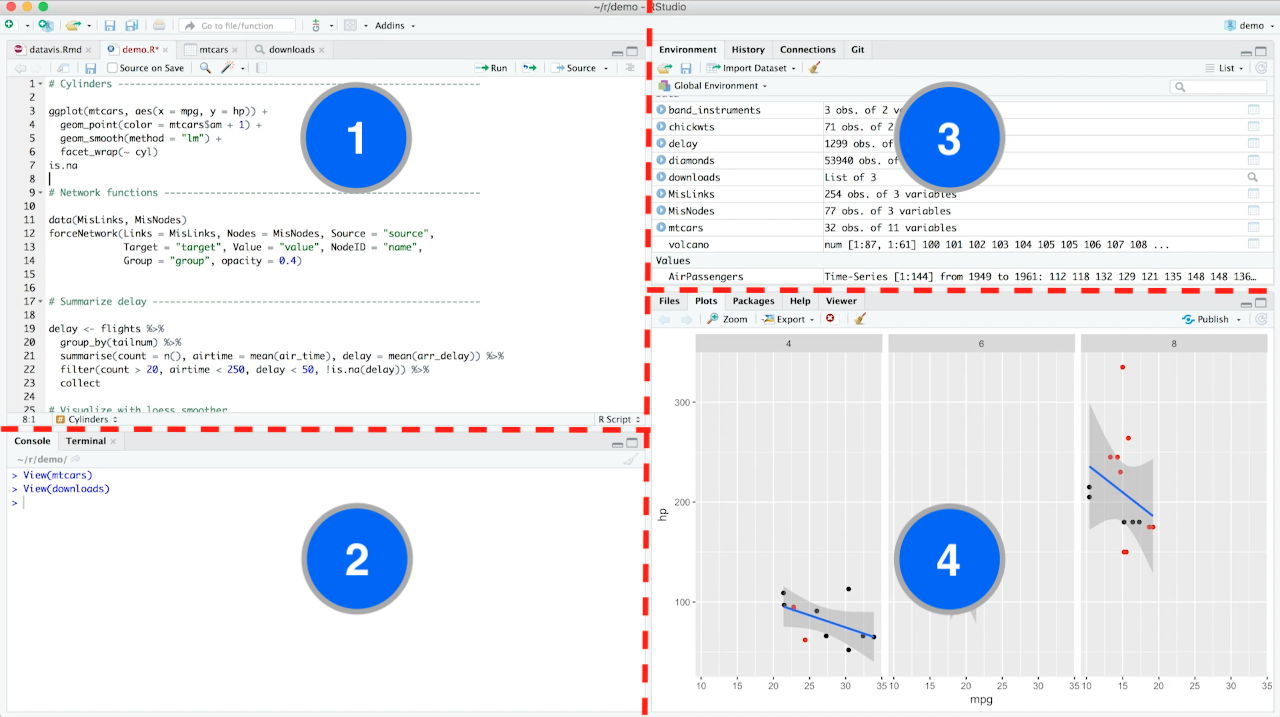
\includegraphics[width=1\linewidth]{images/RStudio} \caption{RStudio Interface terdiri empat bagian utama.}\label{fig:RStudio}
\end{figure}

Seperti dapat dilihat pada gambar \texttt{1.1}. Rstudio memiliki empat
bagian yang memiliki fungsi masing-masing. Bagian pertama (1): digunakan
untuk menulis script dan memiliki beberapa tombol. Untuk menjalankan
script bisa klik run pada bagian kanan atas. Bagian kedua (2) :
merupakan bagian \emph{console} di mana kita bisa melihat script yang
dijalankan. Bagian ketiga (3): merupakan bagian environment, dimana pada
bagian tersebut terdapat beberapa bagian yang bisa pilih. Misalnya,
bagian \texttt{Environment} untuk menampilkan data yang dimasukkan
(diimport), bagian \texttt{Hystory} untuk melihat aktivitas yang sudah
dilakukan dalam satu sesi R, dan bagian \texttt{Connection} untuk
melihat dan mengatur koneksi R dengan database seperti \texttt{SQL} atau
\texttt{SPARK}.

Bagian terakhir (4): berfungsi untuk menampilkan hasil visualiasi
(\texttt{plot}). Selain itu, pada bagian ini kita juga bisa melihat
repository dan file-file yang ada di dalamnya. Lebih penting lagi, di
sini kita juga dapat menemukan bantuan ketika kita lupa instruksi yang
dibutuhkan. Untuk menemukan bantun atau penjelasan kita dapat
menggunakan fungsi \texttt{?} diikuti dengan objek yang ingin dilihat.
Contohnya adalah sebagai berikut.

\begin{Shaded}
\begin{Highlighting}[]
\NormalTok{?read.csv}
\end{Highlighting}
\end{Shaded}

Dengan menuliskan code di atas pada bagian \texttt{console} dan menekan
\texttt{Enter} pada bagian 4 akan menampilkan hasilnya. Di mana pada
tampilan tersebuk kita bisa mendapatkan definisi fungsi sekaligus contoh
penggunaannya. Selain itu, anda juga perlu mencoba untuk menggunakan
fungsi bantuan lainnya, yaitu \texttt{help()} pada console dan lihat apa
yang dihasilkan.

Sebagai rangkuman, pada bagian ini kita sudah mengetahui dan mengenal
beberapa bagian. Pertama untuk menggunakan \texttt{RStudio} kita
terlebih dahulu perlu menginstall \texttt{R}. Untuk mendapatkan bantuan
penjelasan kita bisa menggunakan fungsi \texttt{help()} atau \texttt{?}
diikuti objek yang ingin dilihat. Rstudi terdiri dari beberapa. Untuk
ini saya sarankan untuk mengeksplorasinya lebih jauh, karena pada bagian
selanjutnya kita akan mulai belajar untuk menulis dan menjalankan
script.

\hypertarget{mengunduh-dan-menginstall}{%
\section{Mengunduh dan menginstall}\label{mengunduh-dan-menginstall}}

\hypertarget{mulai-menulis-skrip}{%
\section{Mulai Menulis Skrip}\label{mulai-menulis-skrip}}

\hypertarget{impor-dan-ekspor-data}{%
\section{Impor dan Ekspor Data}\label{impor-dan-ekspor-data}}

\hypertarget{proses-ekstraksi-informasi}{%
\chapter{Proses Ekstraksi Informasi}\label{proses-ekstraksi-informasi}}

Here is a review of existing methods.

\hypertarget{praktik}{%
\chapter{Praktik}\label{praktik}}

\hypertarget{mendapatkan-data}{%
\section{Mendapatkan data}\label{mendapatkan-data}}

\hypertarget{eksplorasi-data}{%
\section{Eksplorasi data}\label{eksplorasi-data}}

\hypertarget{contoh-hasil-kerja}{%
\chapter{Contoh hasil kerja}\label{contoh-hasil-kerja}}

We have finished a nice book.

\hypertarget{sumber-belajar-mandiri}{%
\chapter{Sumber Belajar Mandiri}\label{sumber-belajar-mandiri}}

Some \emph{significant} applications are demonstrated in this chapter.

\hypertarget{example-one}{%
\section{Example one}\label{example-one}}

\hypertarget{example-two}{%
\section{Example two}\label{example-two}}

\bibliography{book.bib,packages.bib}


\end{document}
